\newpage
\title{LEZIONE 2 11/03/2020}\newline
\textbf{link} \href{https://web.microsoftstream.com/video/c3fbadab-4a18-4fbd-bd5c-3a50914235b4?list=user&userId=faa91214-a6f5-40d7-8875-253fd49b8ce1}{clicca qui}
\section{Sistemi dinamici (SD)} 
\subsection{Introduzione}
[immagine dagli appunti del prof]
\begin{center}
    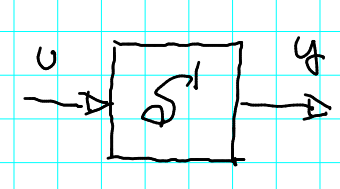
\includegraphics[height=3cm]{../lezione2/img1.PNG}
\end{center}
Premettendo che per questa trattazione la presenza del disturbo non è influente, ci poniamo la seguente domanda: dato un sistema $S$, se conosco l'andamento del sengale di ingresso $u(t)$ sull'intervallo $[t_0, t]$, questo mi basta per conoscere $y[t_0,t]$, cioè l'andamento del segnale di uscita $y(t)$ nell'intervallo $[t_0,t]$?\newline
\newline
Se la risposta a questa domanda è sì, significa che siamo in presenza di un sistema non dinamico, se la risposta è no, il sistema è dinamico.\newline
\newline
Un \textbf{sistema dinamico} (SD) è un sistema in cui la conoscenza degli ingressi su un intervallo di tempo non è sufficiente per determinare l'andamento delle uscite sullo stesso intervallo di tempo.
\subsection{Esempi}
\textbf{es.} sistema non dinamico:\newline
[immagine dagli appunti del prof]
\begin{center}
    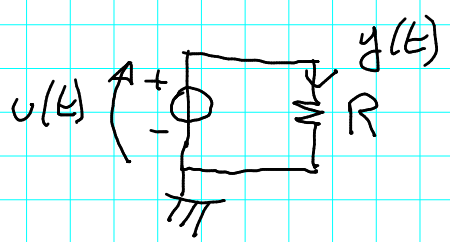
\includegraphics[height=3cm]{../lezione2/img2.PNG}
\end{center}
La tensione $u(t)$ è l'ingresso, la corrente sulla resistenza $R$ è l'uscita $y(t)$. La legge che governa questo circuito è $y(t) = \frac{1}{R}u(t)$, quindi noto $u(t)$ conosco $y(t)$. Siamo in presenza di un sistema non dinamico.\newline
\rule{\textwidth}{0,4pt}
\newline
\newline
\textbf{es.} sistema dinamico:\newline
[immagine dagli appunti del prof]
\begin{center}
    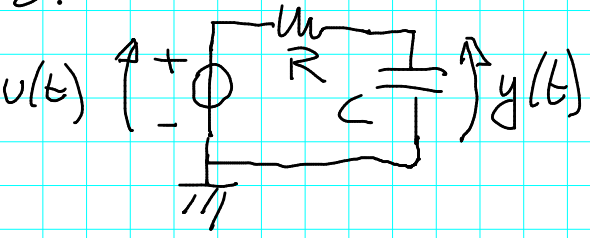
\includegraphics[height=3cm]{../lezione2/img3.PNG}
\end{center}
La tensione $u(t)$ è l'ingresso, la corrente sulla capacità $C$ è l'uscita $y(t)$. Per conoscere $y[t_0,t]$ mi occorrono $u[t_0,t]$ e $y(t_0)$ (lo stato iniziale del condensatore), notiamo che ci serve un solo numero (l'equazione differenziale che governa questo sistema è del primo ordine, quindi necessità di una sola costante arbitraria). Siamo in presenza di un sistema dinamico.\newline
\rule{\textwidth}{0,4pt}
\newline
\newline
\textbf{es.} sistema dinamico:\newline
[immagine dagli appunti del prof]
\begin{center}
    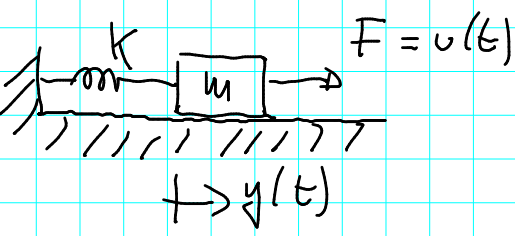
\includegraphics[height=3cm]{../lezione2/img4.PNG}
\end{center}
E' lo stesso esempio visto alla lezione precedente (massa-molla). Per conoscere $y[t_0,t]$ mi occorrono $u[t_0,t]$ e la posizione e la velocità iniziali, notiamo che ci servono due numeri (l'equazione differenziale che governa questo sistema è del secondo ordine, quindi necessità di due costanti arbitrarie). Siamo in presenza di un sistema dinamico.\newline
\rule{\textwidth}{0,4pt}\newline
\newline
\textbf{es.} sistema dinamico:\newline
Prendiamo come esempio un tram che fa delle fermate numerate da $0, \dots, N$. Abbiamo un indice $k$ che indica la fermata corrente, definiamo con $u(k)$ la differenza fra il numero di passeggeri saliti e il numero di passeggeri scesi alla fermata $k$ e con $y(k)$ il numero di passeggeri a bordo quando il tram lascia la fermata $k$. Siamo in presenza di un sistema dinamico, perchè per conoscere $y[k_0,k]$ mi occorrono $u[k_0,k]$ e $y(k_0)$, notiamo che ci serve un solo numero.\newline
\rule{\textwidth}{0,4pt}\newline
\newline
\textbf{es.} sistema dinamico:\newline
[immagine dagli appunti del prof]
\begin{center}
    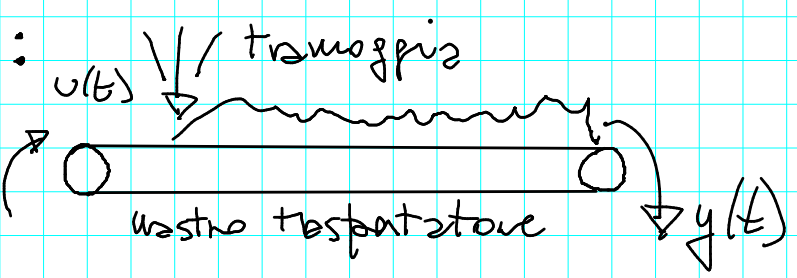
\includegraphics[height=3cm]{../lezione2/img5.PNG}
\end{center}
Supponiamo di avere un nastro trasportatore, sopra il quale c'è una tramoggia che fa cadere del granulato. Definiamo come $u(t)$ la portata in ingresso in $[kg/s]$. Il granulato viene trasportato dal nastro finchè non cade e definiamo come $y(t)$ questa portata in uscita. Diciamo che il tempo di transito sul nastro trasportatore $\tau$ è costante.\newline
Per conoscere $y[t_0,t]$ mi occorerrà analizzare la portata $u[t_0-\tau,t-\tau]$ (notare i $\tau$) e\dots, in questo caso notiamo che ci servono informazioni su un intervallo di tempo diverso da quello desiderato ($[t_0,t]$). Per proseguire nell'esempio in maniera più semplice non utiliziamo $u[t_0-\tau,t-\tau]$, ma utiliziamo un approccio del tutto analogo: per conoscere $y[t_0,t]$ mi occorrono $u[t_0,t]$ e $y[t_0-\tau,t_0]$, che rappresenta cosa c'era sul nastro. Comunque notiamo che, senza fissarci in maniera troppo pignola su questo esempio, diversamente dagli esempi precedenti, la condizione iniziale del sistema sono infiniti numeri, che è ciò che succede quando un sistema è ritardato.\newline
Siamo in presenza di un sistema dinamico.\newline
\rule{\textwidth}{0,4pt}\newline
\newline
Quindi un sistema dinamico, per conoscere l'andamento dell'uscita, ha bisogno di conoscere l'andamento dell'ingresso e il valore iniziale di qualcos'altro (variabili di stato), che solitamente è un numero finito di numeri, ma può anche essere un numero infinito se si è in presenza di un ritardo.\newline
\newline
\textbf{es.} caso particolare:\newline
Prendiamo in considerazione un sistema costituito da un pulsante e una lampadina e il cui funzionamento segue il seguente meccanismo: quando si rilascia il pulsante la lampada cambia stato (si accende se era spenta e viceversa).\newline
Per conoscere l'andamento dell'accensione $y$ nell'intervallo $[t_0,t]$ occorre conoscere l'ingresso (istanti di rilascio del pulsante entro $[t_0,t]$) e lo stato iniziale della lampada, che non rappresenta un numero, ma una variabile booleana. Non sarebbe sbagliato dire che lo stato iniziale della lampada è un numero, ma lo indichiamo come variabile booleana, per mostrare in maniera marcata che non è una variabile di cui si può fare una derivata temporale, l'intero sistema non è governato da un equazione differenziale.\newline
\textbf{oss.} Se mi interessa soltanto lo stato della lampada all'isante $t$, l'informazione che mi occorre è lo stato della lampada a $t_0$ e se il numero di volte in cui il pulsante è stato rilasciato è pari o dispari.\newline
\rule{\textwidth}{0,4pt}\newline
\newline
Tutti questi esempi mostrano i vari sistemi che esistono, noi ci specializzeremo in due classi di sistemi dinamici, quelli a tempo continuo e quelli a tempo dinamico.
\subsection{Sistema dinamico (SD) a tempo continuo (TC)}
Le quantità di cui occorre il valore iniziale per conoscere l'uscita, noto l'ingresso, si dicono \textbf{variabili di stato} e si indicano tipicamente con $x$.
\[
    \begin{rcases}
        x(t_0)\\
        u[t_0,t]
    \end{rcases} \rightarrow x(t), y(t) \;\text{su}\; [t_0,t] \;\;\;t \in \mathbb{R}
\]
In questo corso consideriamo (quasi) sempre sistemi dinamici con solo un ingresso e solo un'uscita, i quali si dicono \textbf{SISO} (Single Input, Single Output), quindi non lavoriamo con vettori, ma con numeri scalari.\newline
\newline
Nel caso a TC abbiamo
\begin{itemize}
    \item $t \in \mathbb{R}$ (scalare)
    \item $u,y \in \mathbb{R}$ (scalari)
    \item $x \in \mathbb{R}^n$ (non per forza uno scalare, può essere un vettore) (come esempio di caso vettoriale si può usare il terzo visto nella sezione precedente, che aveva bisogno di due variabili di stato: posizione e velocità)
\end{itemize} 
dove con $n$ si intende il numero di variabili di stato, (quasi) sempre finito, che prende il nome di \textbf{ordine}.\newline
\newline
\textbf{oss.} Un sistema dinamico è definito su un campo, per noi in $\mathbb{R}$.
\subsubsection{Espressione del sistema}
Il volore assunto dalla prima variabile di stato $x_1(t)$ all'istante $t$ è una funzione $\phi_1(x_1(t),x_2(t),$ $\dots, x_n(t), u[t_0,t], t)$, quindi dipende da sè stessa e da tutte le altre variabili di stato, da  $u[t_0,t]$ e dal tempo $t$ se il sistema è tempo variante. E così pure per le altre variabili di stato:
\[
    \begin{rcases}
        x_1(t) &= \phi_1(x_1(t_0),x_2(t_0), \dots, x_n(t_0), u[t_0,t], t)\\
        \dots \;\;\;&= \;\;\;\dots\\
        x_n(t) &= \phi_n(x_1(t_0),x_2(t_0), \dots, x_n(t_0), u[t_0,t], t)
    \end{rcases} \rightarrow \text{funzioni di transizione dello stato}\;
\]
Queste espressioni prendono il nome di \textbf{funzioni di transizione dello stato}.
\[
    \begin{rcases}
        \\
        \;\;\;\; y(t) = \gamma(x_1(t),x_2(t), \dots, x_n(t), u(t), t)\\
        \\
    \end{rcases} \rightarrow \text{equazione o trasformazione d'uscita}\;
\]
Questa espressione prende il nome di \textbf{equazione o trasformazione d'uscita}.\newline
\newline
La differenza fra $\phi$ e $\gamma$ è che $\gamma$ è una semplice funzione a cui noi diamo dei parametri e ci viene restituita la $y$, mentre le $\phi$ sembrano "qualcosa di strano" che ci richiede la "storia" del sistema come parametri.\newline
\newline
Tutte queste espressioni possono sostanziarsi matematicamente in diversi modi. Vediamo quello principale e il solo di nostro interesse.\newline
\newline
Nei sistemi dinamici a tempo continuo:
\[
    \begin{rcases}
        \dot{x}_1(t) &= f_1(x_1(t),x_2(t), \dots, x_n(t), u(t), t)\\
        \dots \;\;\;&= \;\;\;\dots\\
        \dot{x}_n(t) &= f_n(x_1(t),x_2(t), \dots, x_n(t), u(t), t)
    \end{rcases} \rightarrow \text{equazioni (differenziali) di stato}\;
\]
Queste espressioni prendono il nome di \textbf{equazioni (differenziali) di stato}.
\[
    \begin{rcases}
        \\
        \;\;\;\; y(t) = g(x_1(t),x_2(t), \dots, x_n(t), u(t), t)\\
        \\
    \end{rcases} \rightarrow \text{equazione o trasformazione d'uscita}\;
\]
Quello che è cambiato rispetto a prima è che siamo in presenza di un equazione differenziale e quindi, quando noi integriamo questa equazione differenziale, il valore della funzione dipende da tutta la storia del termine noto.\newline
\newline
Espressione vettoriale:
\[
    x(t) = \left[\begin{matrix}
        x_1(t)\\
        \dots\\
        x_n(t)
    \end{matrix}\right] \Rightarrow  \begin{cases}
        \dot{x}(t) = f(x(t), u(t),t)\\
        y(t) = g(x(t),u(t),t)
    \end{cases} \;\;\;\;u,y \in \mathbb{R}, \;\;\;x \in \mathbb{R}^n
\]
\subsubsection{Definizioni}
\begin{itemize}
    \item Se $f$ e $g$ sono lineari in $x$ e in $u$, allorà dirò che il sistema dinamico è \textbf{lineare}.
    \item Se $f = f(x,u)$ (non compare esplicitamente $t$) e $g = g(x,u)$ (non compare esplicitamente $t$), allora dirò che il sistema dinamico è \textbf{tempo invariante o stazionario}.
    \item Se $g = g(x,t)$ (non compare $u$), allora dirò che il sistema dinamico è \textbf{strettamente proprio}.
\end{itemize}
\subsubsection{Esempi}
Rivediamo alcuni degli esempi di prima ed altri nuovi analizzandoli con le definizioni e i concetti appena introdotti.\newline
\newline
\textbf{es.} esempio del condensatore:\newline
Equazione della maglia $x + Ri = u$ e equazione del condensatore $i = C \dot{x}$.\newline
$$
\begin{cases}
    x + RC \dot{x} = u\\
    y=x
\end{cases} \;\;\;\;\;\begin{cases}
    \dot{x} = -\frac{1}{RC}x + \frac{1}{RC} u\\
    y = x
\end{cases} \;\;\;\;\; f(x,u) = -\frac{1}{RC}x + \frac{1}{RC} u \;\;\text{e}\;\; g(x,u) = x
$$
Evidentemente questo è un sistema dinamico, è lineare, è tempo invariante, è del prim'ordine (una equazione di stato), è strettamente proprio.\newline
\rule{\textwidth}{0,4pt}\newline
\newline
\textbf{es.} Massa-molla:\newline
Nell'esempio di prima eravamo arrivati a dire che $m \ddot{y} = F - ky - h \dot{y}$, dove $F = u$.\newline
A questo punto aggiungiamo che $x_1 = \; \text{posizone}\; = y$ e $x_2 = \; \text{velocità}\; = \dot{y}$, da cui deduciamo che $m \dot{x}_2 = u - k x_1 - h x_2$ e $\dot{x}_1 = x_2$. \newline
Mettendo tutto assieme ottengo:
\[
    \begin{cases}
        \dot{x}_1 = x_2\\
        \dot{x}_2 = -\frac{k}{m} x_1 - \frac{h}{m}x_2 + \frac{1}{m} u\\
        y = x_1
    \end{cases}
\]
Questo è un sistema dinamico, è lineare, è tempo invariante, è strettamente proprio, è del secondo ordine.\newline
\rule{\textwidth}{0,4pt}\newline
\newline
\textbf{es.} nuovo esempio:\newline
[immagine dagli appunti del prof]
\begin{center}
    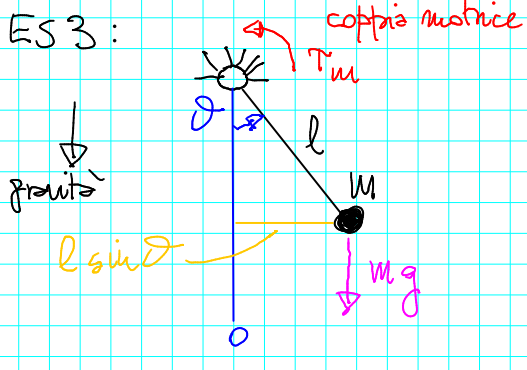
\includegraphics[height=5cm]{../lezione2/img6.PNG}
\end{center}
Il sistema è composta da una cerniera a cui è attaccato un pendolo (un'asta lunga $l$ (senza peso) con attaccato un peso $m$). $\theta$ è l'angolo di sfasamento del pendolo rispetto all'asse verticale. Diciamo che su questo oggetto c'è una coppia (sinonimo di momento) motrice, che chiamo $\tau_m$.\newline
L'equazione che governa questo oggetto è $j = \ddot{\theta} = \sum \text{coppie}\;$, dove $j$ è il momento di inerzia e $\ddot{\theta}$ è l'accellerazione angolare. In questo ingresso ci sono diverse coppie: $\tau_m =$ coppia motrice, il nostro ingresso $= u$, $\tau_f= $ coppia d'attrito $=-h \dot{\theta}$ ($h>0$), $\tau_g =$ coppia gravità $= mg \cdot  l sin(\theta)$ ($mg$ forza di gravità e $l sin(\theta)$ è il braccio).\newline
Quindi $x_1 = \theta$ e $x_2 = \dot{\theta} = \dot{x}_1$.\newline
Il momento di inerzia è $m l^2$.\newline
Quindi riscrivendo l'equazione che governa il sistema otteniamo: $m l^2 \dot{x}_2 = u - h x_2 - m g \cdot l sin(x_1)$.
\[
    \begin{cases}
        \dot{x}_1 = x_2\\
        \dot{x}_2 = - \frac{g}{l} sin(x_1) - \frac{h}{ml^2}x_2 + \frac{l}{ml^2}u\\
        y = x_1
    \end{cases}
\]
Questo è un sistema dinamico, è tempo invariante, è non lineare (per via del termine $sin(x_1)$), è strettamente proprio, è del secondo ordine.\newline
\rule{\textwidth}{0,4pt}
\subsection{Sistema dinamico (SD) a tempo discreto (TD)}
Per tempo discreto si intende che l'evoluzione temporate è "a passi", esiste infatti un indice temporale $k$ intero che tiene traccia dei numeri di passi. In alcuni casi fra $k$ e il tempo $t$ esiste una relazione, nel senso che $k$ rappresenta un intervallo temporale.
\subsubsection{Espressione del sistema}
Come sarà fatto un sistema dinamico a tempo discreto?
\[
    \begin{rcases}
        x_1(k) &= \phi_1(x_1(k_0),x_2(k_0), \dots, x_n(k_0), u[k_0,k], k)\\
        \dots \;\;\;&= \;\;\;\dots\\
        x_n(k) &= \phi_n(x_1(k_0),x_2(k_0), \dots, x_n(k_0), u[k_0,k], t)
    \end{rcases} \rightarrow \text{funzioni di transizione dello stato}\;
\]
Queste espressioni prendono il nome di \textbf{funzioni di transizione dello stato}.\newline
\[
    \begin{rcases}
        \\
        \;\;\;\; y(k) = \gamma(x_1(k),x_2(k), \dots, x_n(k), u(k), k)\\
        \\
    \end{rcases} \rightarrow \text{equazione o trasformazione d'uscita}\;
\]
Queste espressioni prendono il nome di \textbf{equazione o trasformazione d'uscita}.\newline
\newline
E' la stessa identica cosa scritta per i sistemi dinamici a tempo continuo, solo che invece di $t$ abbiamo $k$.\newline
\newline
Anche qui ci domandiamo come effettivamente sostanziare queste formule a livello pratico. Nel caso a tempo continuo abbiamo usato le equazioni differenziali. Nel caso a tempo discreto, invece, usiamo le \textbf{equazioni (di stato) alle differrenze} grazie al concetto di "passo prima", cioè del passo $k-1$ (capiremo perchè più avanti nel corso).\newline
\newline
Nei sistemi dinamici a tempo discreto: 
\[
    \begin{rcases}
        \dot{x}_1(k) &= f_1(x_1(k-1),x_2(k-1), \dots, x_n(k-1), u(k-1), k)\\
        \dots \;\;\;&= \;\;\;\dots\\
        \dot{x}_n(k) &= f_n(x_1(k-1),x_2(k-1), \dots, x_n(k-1), u(k-1), k)
    \end{rcases} \rightarrow \text{equazioni (di stato) alle differrenze}\;
\]
\[
    \begin{rcases}
        \\
        \;\;\;\; y(k) = g(x_1(k),x_2(k), \dots, x_n(k), u(k), k)\\
        \\
    \end{rcases} \rightarrow \text{equazione o trasformazione d'uscita}\;
\]
Nel caso a tempo continuo usavamo l'integrazione per esprimere la dipendenza dagli stati passati, qui abbiamo un equivalente a tempo discreto, in cui lo stato attuale ($k$) dipende dallo stato di prima ($k-1$).
\subsubsection{Definizioni}
Le definizioni di \textbf{lineare}, \textbf{tempo invariante}, \textbf{strettamente proprio}, \textbf{ordine}, sono le stesse di quelle a tempo continuo (sostituendo $t$ con $k$).
\subsubsection{Esempi}
Anche per tempo discreto, come abbiamo fatto per il tempo continuo, rivediamo uno degli esempi già visti la lezione scorsa, analizzandolo con le definizioni e i concetti appena introdotti.\newline
\newline
\textbf{es.} Esempio del tram:\newline
$y(k) = x(k) =$ numero di passeggeri a bordo alla partenza dalla fermata $k$.\newline
$u(k)$ = numero di passeggeri saliti - numeri di passeggeri scesi alla fermata $k$.\newline
Vediamo la legge che governa questo sistema:
\[
        x(k) = x(k-1) + u(k)
\]
\textbf{oss.} non è un eq. di stato ben posta perchè a secondo membro c'è $u(k)$ (e non $u(k-1)$ come vorremmo).\newline
\newline
Per capire bene perchè questa equazione di stato non è corretta vediamo un gioco di ragionamento - o come lo chiama il prof: "educational game":\newline
\newline
Definisco un operatore "anticipo di un passo" e lo chiamo $z$, cioè, quando scrivo $z[v(k)]$ (qualunque cosa sia $v$), intendo in realtà dire $v(k+1)$. Questo operatore è lineare: $z (a v_1(k) + b v_2(k)) = a v_1(k+1) + b v_2(k+1) = a (z(v_1(k)) + b (z(v_2(k))))$.\newline
Tornando al sistema: $y(k) = x(k) = x(k-1) + u(k)$, siccome questo sistema è tempo invariante la stessa cosa succede anche se sposto l'indice di un'unità, quindi posso riscrivere quest'equazione come $x(k+1) = x(k) + u (k+1)$. Ora posso usare il nostro operatore $z$ e scrivere $zx(k) = x(k) + zu(k)$, $(z-1) x(k) = z u(k)$.\newline
A questo punto posso scrivere $y(k) = \frac{z}{z-1}u(k) = (1+ \frac{1}{z-1})u(k) = \frac{1}{z-1}u(k) + u(k)$, dove chiamando $\xi(k) = \frac{1}{z-1}u(k)$, posso scrivere $\begin{cases}
    \xi(k) = \frac{1}{z-1}u(k)\\
    y(k) = \xi(k) + u(k)
\end{cases}$. Arrivati a questo punto scriviamo $(z-1) \xi (k) = u(k)$ e $\xi(k+1) - \xi(k) = u(k)$. Se sfasiamo indietro l'indice di quest'ultima equazione otteniamo $\begin{cases}
    \xi (k) = \xi(k-1) + u(k-1) \;\; \text{(equzione di stato ben posta, non c'è più $u(k)$)}\;\\
    y(k) = \xi(k) + u(k)
\end{cases}$.\newline
Tutto questo mi evidenzia che il sistema è diamico, lineare tempo invariante, del primo ordine, e non strettamente proprio (compare $u(k)$ nell'equazione d'uscita).\newline
\newline
La ragione per cui il sistema è dinamico è che c'è un legame fra ciò che succede al passo prima rispetto al passo corrente.\newline
\rule{\textwidth}{0,4pt}\newline
\newline
Quindi nel caso a tempo continuo, la ragione per cui il sistema è dinamico è perchè c'è un'equazione differenziale e l'operatore utilizzato era la derivata. Nel caso a tempo discreto abbiamo usato questo operatore $z$, definito da noi.\newline
Questo ci fa capire che andando a lavorare sugli operatori che rendono dinamico un sistema, si può elaborare il sistema stesso in modo da far emergere la sua struttura in termini di equazioni di stato e d'uscita.\newline
\newline